\documentclass[10pt,a4paper]{article}
\usepackage[utf8]{inputenc}
\usepackage[spanish]{babel}
\usepackage{graphicx}
\usepackage{fancyhdr}
\usepackage{amsmath}
\usepackage{amsfonts}
\usepackage{amssymb}
%\usepackage{steinmetz}
\usepackage{circuitikz}
\usepackage[includehead=true,includefoot=true,portrait,top = 1cm]{geometry}
\graphicspath{{./FIGURAS/}}

\newcommand{\mymotor}[2] % #1 = name , #2 = rotation angle
{\draw[thick,rotate=#2] (#1) circle (10pt)
 node[]{$\mathsf M$} 
++(-12pt,3pt)--++(0,-6pt) --++(2.5pt,0) ++(-2.8pt,6pt)-- ++(2.5pt,0pt);
\draw[thick,rotate=#2] (#1) ++(12pt,3pt)--++(0,-6pt) --++(-2.5pt,0) ++(2.8pt,6pt)-- ++(-2.5pt,0pt);
}

\newcommand{\mymotorB}[2] % #1 = name 
{\draw[thick] (#1) circle (12pt)
node[above=-3pt]{$\mathsf M$} ++(-8pt,-3pt)--++(15pt,0);
\draw[thick,dashed] (#1) ++(-8pt,-5pt)--++(15pt,0);
}


%\fancyhf{}
\headsep = 2cm
\lhead{Nombre:}
%\lhead{{\huge\textbf{B}} Nombre:}
\chead{}
\rhead{\includegraphics[scale=0.05]{gallinita.pdf}}
\lfoot{}
\cfoot{}
\rfoot{\today}
\renewcommand{\headrulewidth}{0.1pt}
\renewcommand{\footrulewidth}{0pt}
%\lhead{Nombre:}
%\chead{}
%\rhead{\includegraphics[scale=0.05]{gallinita.pdf}}
%\lfoot{}
%\cfoot{}
%\rfoot{\today}
%\renewcommand{\headrulewidth}{0.1pt}
%\renewcommand{\footrulewidth}{0pt}
\def\labelitemi{$\square$}
\begin{document}
\thispagestyle{fancy}

\section*{Sistemas Dinámicos y Realimentación. Examen E2020 \protect\footnote{Copiar códigos, comentarios y resultados en un documento de word o un pdf.}}

\begin{enumerate}
\item Dos bloques de masa idéntica $m$ están unidos entre sí y a dos paredes opuestas mediante muelles de constante $k$. La figura muestra un esquema del sistema completo. Las líneas de puntos que unen los bloques representan los muelles.

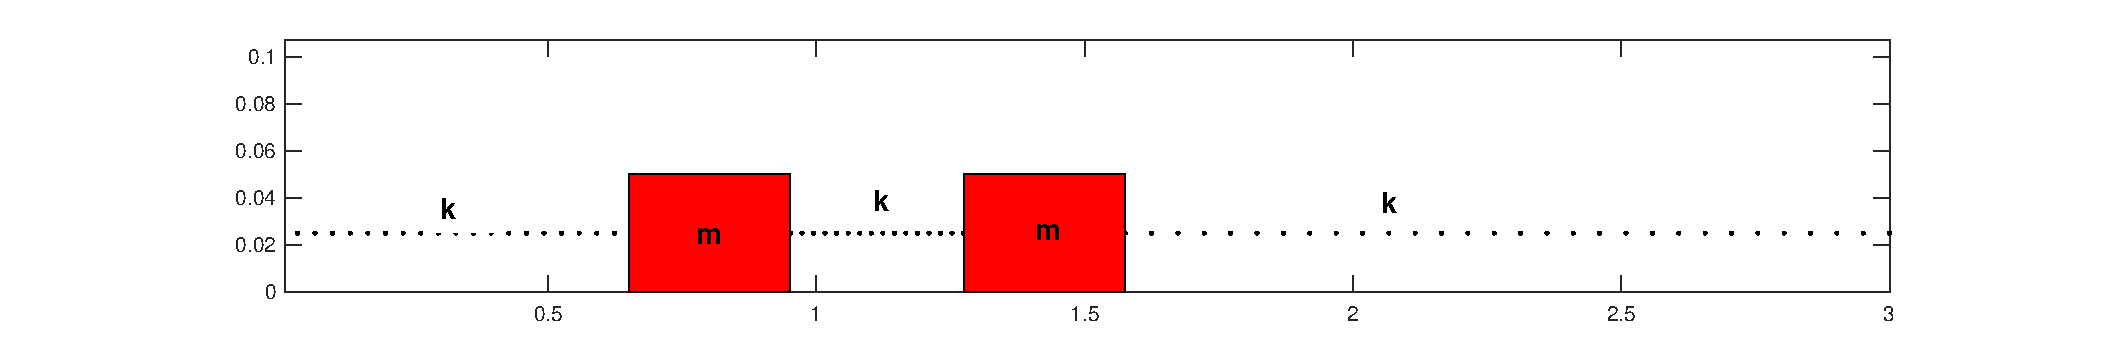
\includegraphics[width=\textwidth]{bloquecitos.eps}
Podemos obtener las ecuaciones del movimiento de los dos bloques en función de su desplazamiento desde su posición de equilibrio:
\begin{align*}
m\frac{d^2\Delta_1}{dt^2} &= -2k\cdot \Delta_1 +k\cdot \Delta_2 -\mu\frac{d\Delta_1}{dt}+F(t)\\
m\frac{d^2\Delta_2}{dt^2} &= -2k\cdot \Delta_2 +k\cdot \Delta_1 -\mu\frac{d\Delta_2}{dt}
\end{align*}

donde $\Delta_1$ y $\Delta_2$ son los desplazamientos de los bloques respecto a su posición de equilibrio y $\mu$ es un coeficiente de fricción igual para ambos bloques. Además, suponemos que es posible ejercer una fuerza externa sobre uno de los bloques, (bloque 1), pero no sobre el otro.
\begin{enumerate}
\item Describe el sistema de los bloque mediante variables de estado de modo que $x_1=\Delta_1$, $x_2 =\Delta_2$, $x_3=\dot{\Delta}_1$, $x_4=\dot{\Delta}_2$.
Considera además que la única salida del sistema es la posición del bloque 2.  
\item Comprueba que el sistema es controlable y diseña un sistema de estabilización por realimentación de estado de modo que los polos estén situados en $[-1, -1, -2, -2]$. Compara la respuesta del sistema en lazo abierto con la del sistema realimentado, suponiendo una entrada nula y condiciones iniciales $x_1=0.5$, $x_2=-1$, $x_3=0$, $x_4=0$. Emplea para los parámetros  $m= 1$, $k=3$ y $\mu=1$. 

\item Añade acción directa de modo que el sistema realimentado alcance un valor de consigna prefijado. Comprueba su funcionamiento correcto para una entrada a escalón unitario y condiciones iniciales nulas.

\item Añade al sistema acción integral, de modo que se conserve la posición de los polos de la realimentación de estados calculada anteriormente.

\item Diseña un estimador de modo que sus polos estén desplazados cuatro unidades hacia a la izquierda respecto a los polos del sistema. Emplea el estimador para realimentar y controlar el sistema. Conserva la acción integral y elimina la acción directa. Comprueba el funcionamiento empleando como entrada un escalón unitario y condiciones iniciales $x_1=0.5$, $x_2=-1$, $x_3=0$, $x_4=0$. Considera nulas las condiciones iniciales del estimador $\hat{x_i}=0$.


\end{enumerate}

\item Tomando como punto de partida la representación en variables de estado del sistema del ejercicio anterior\footnote{Hacerlo todo empleando la representación numérica. En simbólico salen expresiones muy complicadas.}
\begin{enumerate}
\item Obtener los modos normales del sistema, comprobar que loas autovalores del sistema son complejos conjugados dos a dos. Obtener un conjunto de condiciones de modo que cada una excite un solo modo normal. ¿Son realizables físicamente?.
\item Obtener a partir de los resultados obtenidos un nuevo conjunto de condiciones iniciales que de modo que cada una excite a uno de los pares de modos normales complejos conjugados.  
\item Construir una representación diagonal del sistema. Empleando la representación diagonal construida, obtener de forma analítica (empleando \texttt{initial} o \texttt{lsim}) la evolución de los estados para las condiciones iniciales definidas en el apartado anterior. Representarlas gráficamente.  
\item Comparar los resultado obtenidos en el apartado anterior con los que se obtendría para condiciones iniciales arbitrarias. Indica a --a tu juicio-- cuál es la diferencia  más significativa.
\end{enumerate}

\item Una versión normalizada de un modelo de congestión para una red de comunicaciones puede definirse como,
\begin{flalign*}
\dot{x}_1 &= \frac{1}{x_2} - x_1^2 & \\
\dot{x}_2 &=  \frac{x_1}{x_2} -1
\end{flalign*}
Donde $x_1$ representa el tamaño de la ventana de envío y $x_2$ el tamaño del \emph{buffer} empleado por el \emph{router}. (Ambas cantidades deben se mayores que cero para que el modelo tenga sentido.)
\begin{enumerate}
\item Encontrar el punto de equilibrio
\item Linealizar en torno al punto de equilibrio y estudiar su estabilidad.
\item Empleando como función de Lyapunov, 
\begin{flalign*}
V &= (x_1-x_{e1})^2 + (x_2-x_{e2})^2 &
\end{flalign*}
donde $[x_{e1},x_{e2}]$ son las coordenadas del punto de equilibrio, discutir su estabilidad. (Nota: Solo tiene sentido discutirla para la región del espacio de fase en que el sistema está definido. Si no resulta fácil hacerlo analíticamente, también vale hacer un dibujo de la derivada de Lyapunov en torno al punto de equilibrio para apoyar la discusión.)
\end{enumerate}
\end{enumerate}
\end{document}
